\documentclass[11pt]{article}
\usepackage{graphicx}
\usepackage{hyperref}
\usepackage{caption}
\usepackage{amsmath}
\usepackage{mathtools}
\usepackage{physics}
\usepackage{listings}
\usepackage{xcolor}
\usepackage{subfig}
\newcommand{\numpy}{{\tt numpy}}    % tt font for numpy

\topmargin -.5in
\textheight 9in
\oddsidemargin -.25in
\evensidemargin -.25in
\textwidth 7in

\graphicspath{ {./imgs/}
               {../} }

\begin{document}

% ========== Edit your name here
\author{Due on April 8, 2022}
\title{CS 498: Assignment 4: Segmentation}
\date{March 25, 2022}
\maketitle

\medskip


\section*{Submission}
In this assignment, you will implement semantic segmentation using neural networks. The starter code consists of an iPython notebook "mp4.ipynb" which can be opened and run on Google colab. Please put together a single PDF with your answers and figures for each problem, and submit it to Gradescope (Course Code: JBXJVZ). 
We recommend you add your answers to the latex template files we provided. More details on what to report are in the provided notebook. 

Reminder: please put your name and netid in your pdf.
Your submission should include your pdf and filled out mp4.ipynb.

\section*{Semantic Segmentation} 

\paragraph{Question 1 (Data loading and augmentation)[1 pt]:}
We provide code that loads the segmentation data. In this part you will need to perform data augmentation on the loaded data within the "SegmentationDataset" class. In particular you should take a random crop of the image and with some probability you should flip the image horizontally. You should experiment with different probabilities and crop sizes and report the results in your pdf. Make sure to use pytorch built in transforms methods.

\begin{figure}[h]
    \centering
    \subfloat [\centering default]{{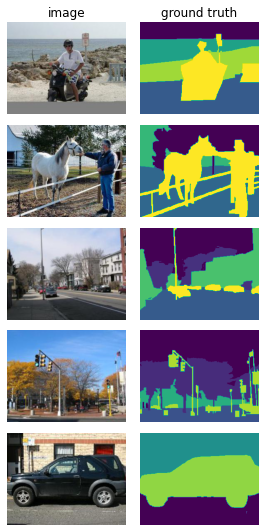
\includegraphics[width=0.24\linewidth]{default.png}}}
    % \quad
    \subfloat [\centering scaling]{{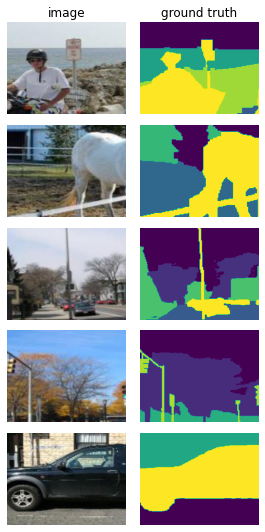
\includegraphics[width=0.24\linewidth]{scale_008_100_ratio_1_flip_0.png}}}
    % \quad
    \subfloat [\centering aspect ratio]{{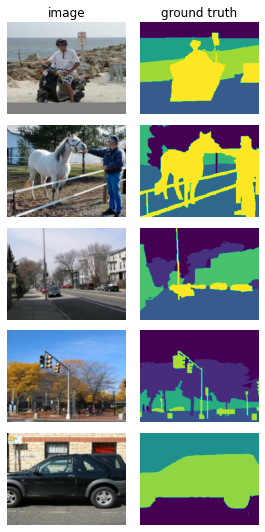
\includegraphics[width=0.24\linewidth]{scale_080_100_ratio_3_4_flip_0.png}}}
    % \quad
    \subfloat [\centering flipping]{{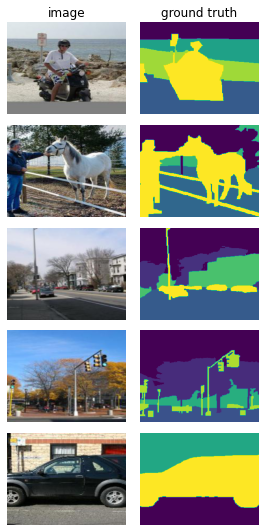
\includegraphics[width=0.24\linewidth]{scale_100_100_ratio_1_flip_50.png}}}
    \caption{Comparisons of image samples when (a) no transform, (b) scaling, (c) change in aspect ratio, and (d) horizontal flipping is applied.}
    \label{fig:transform}
\end{figure}

\paragraph{Question 2 (Simple Baseline) [2 pts]:} 
In this part you will be modifying "simple\_train" and "simple\_predict". For each pixel you should compute the distribution of class labels at that pixel from the training dataset. When predicting classes for a new image, simply output these class frequencies at each pixel. You can run the evaluation code (from the next question) with your simple baseline and see its mean average precision which we provide - it should be around 24.

\begin{figure}[h]
    \centering
    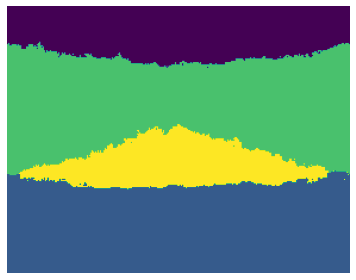
\includegraphics[width=0.5\linewidth]{simple_predict.png}
    \caption{Results of the simple prediction algorithm.}
    \label{fig:simple-predict}
\end{figure}

\paragraph{Question 3 (Evaluation Metrics) [1 pts]:}  
We must evaluate the quality of our predictions. In this part you will fill in "compute\_confusion\_matrix". You should write code to compute the confusion matrix as well as IoU for the predicted segmentation when compared to ground truth. We provide code for visualizing the computed values as well as computing mean average precision.

\begin{figure}[h]
    \centering
    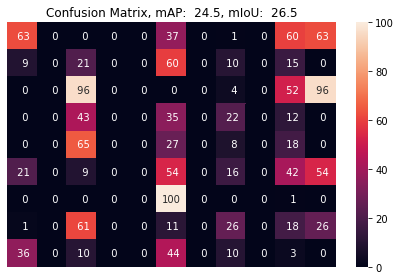
\includegraphics[width=0.5\linewidth]{eval_simple_predict.png}
    \caption{Evaluation on the results of the simple prediction.}
    \label{fig:eval-simple-predict}
\end{figure}

\paragraph{Question 4 (Loss function) [2 pt]:} 
To train a model we need a loss function. In this part you will fill in "cross\_entropy\_criterion" with your implementation of the weighted cross entropy between predicted class probabilities and ground truth class labels.

\paragraph{Question 5 (Train loop) [2 pt]:} 
In this part you will implement the stochastic gradient descent training loop in pytorch, modifying "train". We provide code to validate a trained model and a skeleton for training one. 

\paragraph{Question 6 (Model definition and training) [4 pt]:} 
Implement a basic convolutional neural network, as well as the U-Net architecture for semantic segmentation. Train your models with the code you wrote for Question 5. 

{\centering \tt \small
\# BaseConv \\
sky: AP: 0.95, IoU: 0.90 \\
tree: AP: 0.62, IoU: 0.65 \\
road: AP: 0.90, IoU: 0.78 \\
grass: AP: 0.59, IoU: 0.71 \\
water: AP: 0.18, IoU: 0.45 \\
building: AP: 0.68, IoU: 0.55 \\
mountain: AP: 0.04, IoU: 0.28 \\
foreground: AP: 0.59, IoU: 0.56 \\
misc: AP: 0.01, IoU: 0.06 \\
mean: AP: 0.50, IoU: 0.55 \\

\# UNet \\
sky: AP: 0.95, IoU: 0.87 \\
tree: AP: 0.74, IoU: 0.75 \\
road: AP: 0.93, IoU: 0.81 \\
grass: AP: 0.72, IoU: 0.77 \\
water: AP: 0.29, IoU: 0.57 \\
building: AP: 0.74, IoU: 0.65 \\
mountain: AP: 0.06, IoU: 0.27 \\
foreground: AP: 0.68, IoU: 0.65 \\
misc: AP: 0.01, IoU: 0.09 \\
mean: AP: 0.57, IoU: 0.60 \\
}

\begin{figure}[h]
    \centering
    \subfloat {{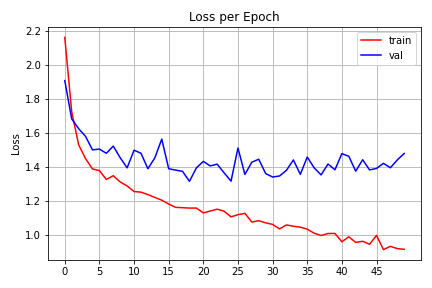
\includegraphics[width=0.45\linewidth]{loss-BaseConv.png}}}
    \qquad
    \subfloat {{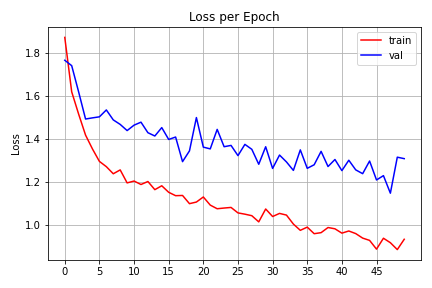
\includegraphics[width=0.45\linewidth]{loss-UNet.png}}}
    \caption{Loss curve of training \texttt{BaseConv} (left) and \texttt{UNet} (right) models, respectively.}
    \label{fig:loss-BaseConv-UNet]}
\end{figure}


\begin{figure}[h]
    \centering
    \subfloat {{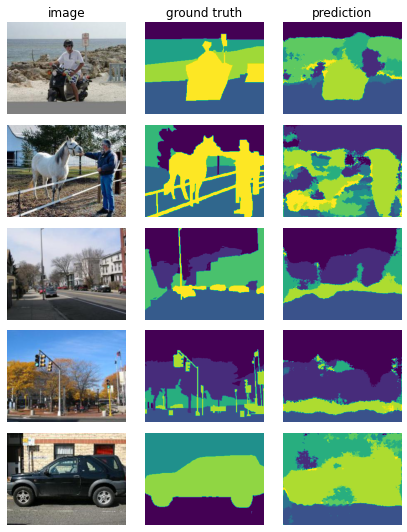
\includegraphics[width=0.45\linewidth]{pred-BaseConv.png}}}
    \qquad
    \subfloat {{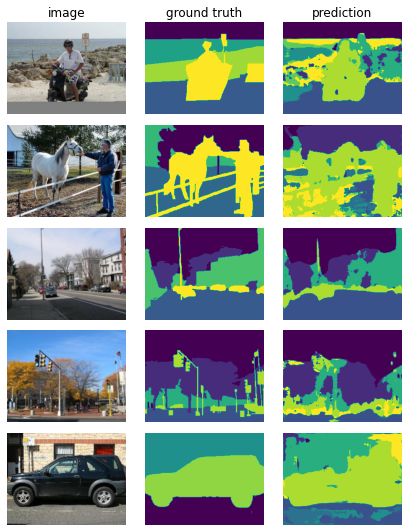
\includegraphics[width=0.45\linewidth]{pred-UNet.png}}}
    \caption{Predictions made by \texttt{BaseConv} (left) and \texttt{UNet} (right) models, respectively.}
    \label{fig:pred-BaseConv-UNet]}
\end{figure}




\paragraph{Question 7 (Use Pretrained Model) [3 pt]:} 
In this part you will build on resnet-18 (note there are multiple ways to do this). Report your results, they should be better than the best you got using UNet training from scratch.

{\centering \tt \small
\# ResnetBasedModel \\
sky: AP: 0.94, IoU: 0.84 \\
tree: AP: 0.75, IoU: 0.80 \\
road: AP: 0.94, IoU: 0.88 \\
grass: AP: 0.36, IoU: 0.50 \\
water: AP: 0.76, IoU: 0.80 \\
building: AP: 0.87, IoU: 0.76 \\
mountain: AP: 0.16, IoU: 0.31 \\
foreground: AP: 0.78, IoU: 0.70 \\
misc: AP: 0.04, IoU: 0.42 \\
mean: AP: 0.62, IoU: 0.67 \\

\# ResnetUNetModel \\
sky: AP: 0.97, IoU: 0.91 \\
tree: AP: 0.81, IoU: 0.77 \\
road: AP: 0.95, IoU: 0.86 \\
grass: AP: 0.59, IoU: 0.65 \\
water: AP: 0.67, IoU: 0.78 \\
building: AP: 0.88, IoU: 0.80 \\
mountain: AP: 0.10, IoU: 0.60 \\
foreground: AP: 0.84, IoU: 0.81 \\
misc: AP: 0.00, IoU: 0.09 \\
mean: AP: 0.65, IoU: 0.70 \\
}

\begin{figure}[h]
    \centering
    \subfloat {{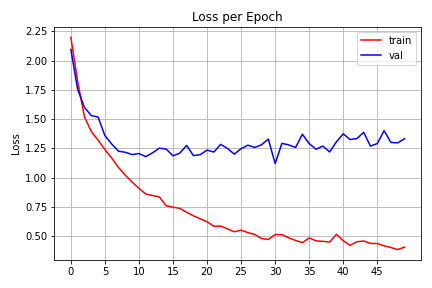
\includegraphics[width=0.45\linewidth]{loss-ResnetBasedModel.png}}}
    \qquad
    \subfloat {{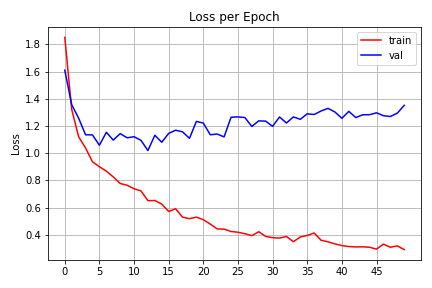
\includegraphics[width=0.45\linewidth]{loss-ResnetUNetModel.png}}}
    \caption{Loss curve of training ResNet-based models without skip connection (left) and with skip connection (right), respectively.}
    \label{fig:loss-ResnetBasedModel]}
\end{figure}


\begin{figure}[h]
    \centering
    \subfloat {{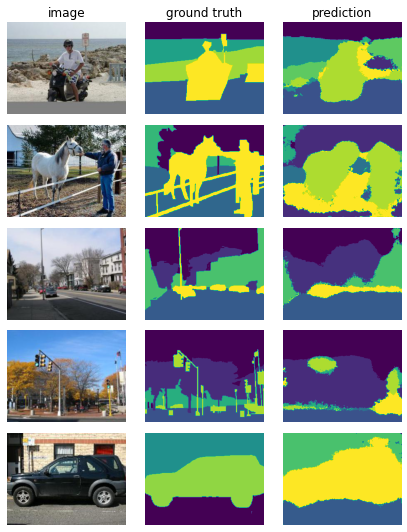
\includegraphics[width=0.45\linewidth]{pred-ResnetBasedModel.png}}}
    \qquad
    \subfloat {{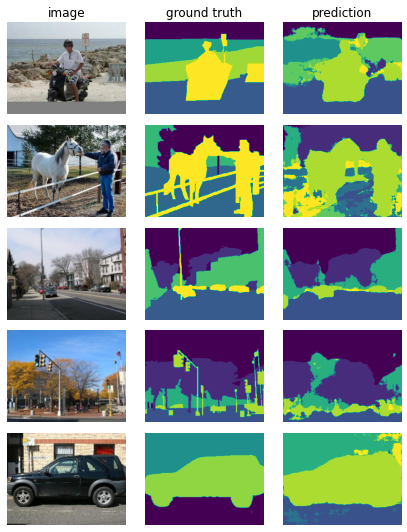
\includegraphics[width=0.45\linewidth]{pred-ResnetUNetModel.png}}}
    \caption{Predictions made by ResNet-based models without skip connection (left) and with skip connection (right), respectively.}
    \label{fig:pred-ResnetBasedModel]}
\end{figure}


\section*{Instance Segmentation (Bonus 4pt)}

Now we have a deep semantic segmentation algorithm. However, the model cannot distinguish each instance. Could you use a similar UNet model to build an instance segmentation algorithm? Please download the Upenn-Fudan pedestrian dataset here \url{https://www.cis.upenn.edu/~jshi/ped_html/} and get their instance labels. There are two types of instance segmentation methods, detection-free or detection-based. Choose either one of them. 

Please refer to the Deep Watershed Transform for an example of detection-free method \url{https://github.com/min2209/dwt}. Your goal is to build a network with two headers, one to predict the binary semantic label similar to your semantic segmentation network and the other to predict the distance transform to the boundary. Once you have these two, the watershed transform could be applied to recover per-pixel instance labels.  

For the detection-based method, please refer to the MaskRCNN (\url{https://pytorch.org/vision/stable/_modules/torchvision/models/detection/mask_rcnn.html}). You will develop a network that predicts detection proposals first. Then within each detection proposal, a binary foreground and background segmentation is conducted to separate each instance. 

For each method, you should implement 1) the loss function the paper uses; 2) implement the data loader and post-processing that converts network output to per-pixel instance label 3) train and evaluation each model (you could either reuse your UNet backbone or follow the original paper). 

\end{document}. 

\grid
\grid